%%%%%%%%%%%%%%%%%%%%%%%%%%%%%%%%%%%%%%%%%%%%%%%%%%%%%%%%%%%%%%%%%%%%%%%%%%%%%%%%
%2345678901234567890123456789012345678901234567890123456789012345678901234567890
%        1         2         3         4         5         6         7         8

\documentclass[a4paper, 10 pt, conference]{ieeeconf}  % Comment this line out
                                                          % if you need a4paper
%\documentclass[a4paper, 10pt, conference]{ieeeconf}      % Use this line for a4
                                                          % paper

\IEEEoverridecommandlockouts                              % This command is only
                                                          % needed if you want to
                                                          % use the \thanks command
\overrideIEEEmargins
% See the \addtolength command later in the file to balance the column lengths
% on the last page of the document




\usepackage{graphics} % for pdf, bitmapped graphics files
\usepackage{epsfig} % for postscript graphics files
\usepackage{mathptmx} % assumes new font selection scheme installed
\usepackage{times} % assumes new font selection scheme installed
\usepackage{amsmath} % assumes amsmath package installed
\usepackage{amssymb}  % assumes amsmath package installed
\usepackage{tabularx}
\usepackage{array}
\usepackage{hyperref}

\title{\LARGE \bf
Data Privacy for Children: Protecting Vulnerable Populations Online
}

%\author{ \parbox{3 in}{\centering Huibert Kwakernaak*
%         \thanks{*Use the $\backslash$thanks command to put information here}\\
%         Faculty of Electrical Engineering, Mathematics and Computer Science\\
%         University of Twente\\
%         7500 AE Enschede, The Netherlands\\
%         {\tt\small h.kwakernaak@autsubmit.com}}
%         \hspace*{ 0.5 in}
%         \parbox{3 in}{ \centering Pradeep Misra**
%         \thanks{**The footnote marks may be inserted manually}\\
%        Department of Electrical Engineering \\
%         Wright State University\\
%         Dayton, OH 45435, USA\\
%         {\tt\small pmisra@cs.wright.edu}}
%}

\author{Surya Teja Kommuguri$^{1}$, Abhinav Tallapragada Srinivasa$^{2}$ and Yaswanth Kumar Lekkala$^{3}$% <-this % stops a space
\\ Masters in Information Technology, ARIZONA STATE UNIVERSITY
\thanks{We would like to Express our Thanks to }% <-this % stops a space
\thanks{$^{}$ Dr. Tatiana Walsh, Chair, Information Technology at Ira A. Fulton Schools of Engineering at Arizona State University.}%
\thanks{$^{}$
        {\tt\small }}%
}


\begin{document}



\maketitle
\thispagestyle{empty}
\pagestyle{empty}


%%%%%%%%%%%%%%%%%%%%%%%%%%%%%%%%%%%%%%%%%%%%%%%%%%%%%%%%%%%%%%%%%%%%%%%%%%%%%%%%
\begin{abstract}

Children's online privacy is increasingly vital as their internet usage rises. This paper examines the risks children face online, the legal frameworks protecting their data, technological solutions, and strategies for promoting digital literacy. Balancing privacy with safety and autonomy is essential for their well-being.

\end{abstract}


%%%%%%%%%%%%%%%%%%%%%%%%%%%%%%%%%%%%%%%%%%%%%%%%%%%%%%%%%%%%%%%%%%%%%%%%%%%%%%%%
\section{INTRODUCTION}

Online world for children is becoming increasingly popular day by day. More and more kids are going online these days. They spend a lot of time on the internet because technology is changing how we live and connect with others. Children's use of the internet has increased dramatically as a result of the popularity of video games, particularly among older kids who wish to play games online.
\subsection{Ensuring children’s privacy online}
Boyd (2014) stated that social media has taken over the internet as the main influence in the last decade. It has changed the way people think about the personal privacy and how they express themselves online. Many people, including children, use it to share information, sometimes directly and sometimes indirectly, including personal details. \textit{“Last, since the rise of search engines, people’s communications are also often searchable”}(Boyd, D., 2014, p. 12). The media often depicts modern children as having unique talents because they’ve grown up with digital technology. They’re appreciated for their ability to multitask and their frequent use of texting. However, there are also worries that these kids are vulnerable to unprecedented new risks: sexual producers, cyberbullying, and numerous forms of intellectual and moral decline, including internet addiction, not paying attention, decreased literacy, reckless oversharing on so on. Navigating the online world safely is crucial for young children and it is public responsibility to protect them from risks.
\textit{“Children are perceived as more vulnerable than adults to privacy online threats due to their lack of digital skills and awareness of privacy risks”} (Stoilova et al., 2019, p. 4). As people become more concerned about keeping children's information safe and not letting companies use it for making money, it's really important to think about how much kids understand about the internet, how good they are at using computers, and whether they can make smart decisions about what they do online. Most of the people in society think about how it’s risky for younger generations to share personal stuff, but it is important to look at digital privacy in a wider way thinking about how it affects a child’s overall health and happiness. Privacy is really important for young people because it lets them have the freedom to figure out who they are without worrying about someone watching or finding out everything about them.
\\ Even though children can gain a lot from being online, there are also several dangers they need to be aware of. These risks come from companies making money off their personal details, the impact sharing too much personal information can have on their reputation and future, and the safety risks they might encounter online. As technology gets better, there's more data that can be gathered about kids from their gadgets and surroundings. When children lose their privacy online, it can harm their dignity and autonomy. This can make it harder for them to freely figure out who they are and to stay anonymous. Besides these direct privacy issues, there's also the risk of other problems like being targeted by online ads and facing safety risks. Some of these dangers might have immediate consequences, while others might affect them later on, but it's important to be aware of them all.
\subsection{Importance of privacy protections for safeguarding children online}
Safeguarding children’s privacy online is crucial for their safety. These protective measures prevent predators from exploiting their personal information, ensuring that they cannot deceive or endanger them. So, by making sure children’s privacy is secure, we can help keep them safe while they’re using the internet. They also reduce the risk of identity theft by controlling the sharing of personal details, thus safeguarding children’s financial security. Privacy protections also contribute in maintaining children’s mental well-being by minimizing exposure to online tracking and profiling.
\\ Finding the right balance between allowing children independence and ensuring their safety can be tricky. However, research shows that providing appropriate support significantly impacts children’s online privacy. While most studies focus on parents, it’s essential to explore how teachers and child support workers can contribute effectively in this area.


\section{Demonstrating Mastery of the Pertinent Security Privacy Material}

\subsection{Addressing New Risks: Safeguarding the Privacy of Vulnerable Children}

When our information is used online, it impacts everyone who uses the internet. This is especially important for groups like children who might not realize the risks of their data being used (Shin and Kang, 2016). A survey done in 2015 by the Global Privacy Enforcement Network (GPEN) checked children's apps and websites to see if they were safe. The survey found that about two-thirds of the 1,494 websites and apps they looked at didn't have any way for kids or their parents to control how much personal information was shared. This shows that kids and their parents don’t always know about the dangers online or understand how the things they share online could be used (Livingstone, Carr and Byrne, 2016; Byrne et al., 2016). 
\\ Most of the companies use children and teenagers as an important market because they influence their families’ buying decisions. Understanding children's online habits and behaviour is valuable to businesses, helping them create effective strategies to reach this significant portion of the online market. Spending time online is a major activity for children today, making them a crucial consumer group. However, this can lead to exploitation of children’s privacy by marketers who observe their online activities and create online environments that appeal to children. This not only affects their privacy but also their access to information, as marketers can shape their online experiences and social environments. For example, partnerships between advertisers and YouTube vloggers often blur the line between genuine content and paid advertising. Research has shown that many companies use popular youtubers to promote their products in videos without clearly disclosing that it’s paid advertising.

\begin{figure}[h]
    \centering
    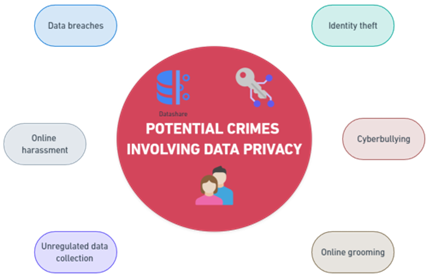
\includegraphics[width=0.5\textwidth]{1.png}
    \caption{Potential risks involving data privacy}
    \label{fig:example}
\end{figure}
Another worrying issue is the increasing use of mass surveillance techniques by certain governments, which collect the personal data of internet users worldwide, including young children. In today's world of technology, the internet offers children great opportunities to learn, but it also means that governments and big companies are watching what they do more closely (Brown and Pecora, 2014). When programmers create new apps or programs, it’s really important to think about privacy right from the start. This means creating them while thinking about privacy and making sure they keep people’s information safe without needing them to do anything extra. This helps make the internet safer for everyone.
\\ In today’s digital world, we worry about things like data breaching, cyberbullying, and exposure to harmful content. These problems affect children and vulnerable groups a lot. To make things safer, we need to work on protecting their privacy better. By focusing on security and teaching people how to stay safe online, one can make the internet a safer place for everyone.



\subsection{Protecting children’s data: legal frameworks}
\subsubsection{Analysis of existing laws and regulations on children’s data privacy}

Looking at the current laws about children’s privacy online, we see a detailed system set up to keep children personal information safe.
The European Union’s General Data Protection Regulation (GDPR) says that companies need permission from parents or legal guardians before using personal information of children under 16 years old. This requirement is consistent in both Germany and Romania. Additionally, the GDPR allows each country to decide if they want to set a lower age limit for consent. Some set of rules imposed by GDPR in the European countries are:
\begin{itemize}
    \item Children should receive information about how their personal data is used in a way that is easy to understand and clear.
    \item Each country can decide to set a lower age for when children can give their own consent. Before using personal information of children under 16, companies must get permission from parents or legal guardians.
    \item Data controllers have the responsibility to make sure that the person giving consent for a child is actually their parent. They must get permission from a legal guardian in a secure way.
    \item National regulators have the authority to impose fines on companies for breaking GDPR rules, with fines reaching up to 4\% of the company's global revenue (Law Library of Congress 2021).
\end{itemize}
Another global initiative is the Children’s Online Privacy Protection Act (COPPA), designed to safeguard the privacy of children under the age of 13. COPPA is applicable to websites and online services tailored for children and utilized for commercial purposes. The important things that a website operator must do according to the Act are:
\begin{itemize}
    \item Creating a thorough privacy policy that explains the information gathered from users.
    \item Obtaining a trusted parent's approval before gathering personal details from a child under 13 years old.
    \item Informing parents about any information gathered about their children by the website.
    \item Making sure that any personal information collected online from children is kept safe and private by protecting its confidentiality, security, and integrity.
\end{itemize}
\subsubsection{Effectiveness of GDPR and COPPA on protecting children}
Both GDPR and COPPA aim to safeguard children's online privacy by imposing legal obligations on organizations to obtain parental consent before collecting or processing personal data. While GDPR applies more broadly to all online services operating within the EU, COPPA specifically targets websites and online services directed towards children under 13 years old, regardless of their geographical location. Enforcement mechanisms and penalties for non-compliance vary between the two regulations but serve the common goal of ensuring accountability and adherence to data protection principles.
\begin{table}[h]
    \centering
    \newcolumntype{C}{>{\centering\arraybackslash}X} % Define centered column type
    \begin{tabularx}{0.5\textwidth}{|C|C|C|} % Use the centered column type
        \hline
        \textbf{Aspect} & \textbf{GDPR (EU)} & \textbf{COPPA (US)} \\
        \hline
        Target Age Group & Children under 16 years old & Children under 13 years old \\
        \hline
        Parental Consent & Required before processing personal data of children & Required before collecting personal information of children \\
        \hline
        Information Provision & Children should receive clear and understandable information & Websites must have comprehensive privacy policies \\
        \hline
    \end{tabularx}
    \caption{International approaches to protecting children’s online privacy}
    \label{tab:example}
\end{table}




\section{Arguing for Your Position}
\subsection{Technical solutions for enhancing children’s privacy: Future trends and challenges}
Some technological solutions aimed at enhancing children’s privacy focus on safeguarding their personal data and online interactions:
\begin{enumerate}
    \item Allow parents to control and monitor their children’s online activities and give limited access to certain websites, tracking location, and monitoring social media usage. 
    \item Implement a blockchain technology to give children more control over personal data and reduce the risk of data breaches.
    \item Develop educational tools by building interactive games to educate children about the importance of privacy and safe online behaviour.
    \item Developing extensions that block tracking scripts, prevent cookies from being stored, and encrypt communications to enhance privacy while browsing.
    \item Provide privacy focused social media platforms that includes features like age verification, moderation and limited data collection.
\end{enumerate}
The increasing popularity of IoT gadgets and wearable for children, such as smartwatches and GPS trackers, has raised concerns about how these devices handle children’s data securely and privately. To address this issue, it’s vital to ensure that data transmission is safeguarded using strong encryption methods. Parents should have full control over how their child’s data is shared. Moreover, companies must be clear and honest about how they gather and utilize children’s data. This transparency helps parents make informed choices about their children's privacy and safety. With the increasing use of AI in products and services for children, there’s a growing need to prioritize privacy in the development of these systems. Meeting data protection regulations is a big challenge for companies in the children’s tech industry. Emerging technologies offer exciting opportunities for children, but they also come with privacy concerns. To address this, privacy features should be built directly into these technologies, and developers need clear guidelines on how to handle children’s data responsibly. However, there are some downsides to keep in mind. Parental control apps, which help parents manage what their children do online, might gather information about the kids. This can make people worry about who can see that info and how they might use it. Also, it takes ongoing work to update educational materials so they stay helpful as privacy risks change. Using privacy-focused technology could mean that apps don’t work as well or might not be as fun to use. So, we need to be careful and keep improving how we protect children’s privacy online.
\subsection{Strategies for promoting digital literacy and responsible online behaviour}
It’s really important for schools to teach kids how to use digital stuff responsibly. When students learn about this in different subjects, they understand better how to stay safe online. This helps them handle both good and bad things on the internet.
\\ Teachers need to learn about digital stuff too so they can teach it well. They should know about digital tools, staying safe online, and how to find good stuff on the internet. Then, they can help students use the internet safely. Having workshops and events for parents and the community is important too. These events give tips on managing kids’ online time, keeping them safe online, and having good online habits at home. When everyone in the community gets involved, schools can make sure everyone knows how to use technology safely.
\\ Making online resources like articles, videos, and quizzes is also helpful. These resources teach people of all ages about staying safe online. Fun websites and apps can make learning about this stuff more interesting too. When these resources are easy to find and use, everyone can feel more confident about using the internet in a smart way.
\begin{figure}[h]
    \centering
    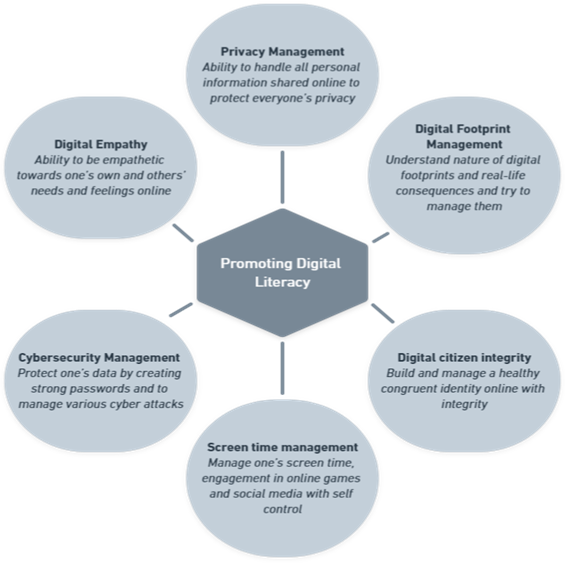
\includegraphics[width=0.4\textwidth]{2.png}
    \caption{Promoting digital literacy}
    \label{fig:example}
\end{figure}
\subsubsection{Encouraging safe internet practices}
Ensuring children’s safety online is all about teaching them how to use the internet responsibly. It’s crucial to help them learn to think carefully about what they see online. This means showing them how to check if something they read or see is true or not, and where to find trustworthy information. By doing this, kids can make smarter choices when they’re browsing the internet. It is important to explain to kids why it’s vital to keep their personal info safe online. This includes things like their name, address, and phone number. Kids should also know how to set privacy settings on apps and websites, and how to spot things like cyberbullying or scams. 
\\ Teaching kids about their “digital footprint” is also essential. That’s the trail of information they leave behind online. Children need to understand that what they do on the internet can affect them later on, so it is important to think before sharing anything personal. Encouraging kids to be kind and respectful online is another crucial aspect. Creating a friendly and safe internet community where everyone feels welcome is important. By teaching kids about these things and giving them the tools to stay safe online, we’re helping them have a better and more secure experience on the internet.
\subsection{Importance of privacy in digital platform design}
Including privacy issues in the design of online platforms is the first step towards guaranteeing the protection of children’s privacy in the digital realm. Maintaining compliance with laws like the Children’s Online Privacy Protection Act (COPPA), fostering user confidence, and promoting appropriate online behaviour all depend on this tactic. One of the primary arguments in favour of giving privacy top priority in platform design is the protection of children’s personal information. Due to their limited understanding of digital privacy, children are particularly vulnerable to threats to their online privacy. Platforms can prevent unauthorised access to sensitive data belonging to minors by putting in place safeguards including strong data encryption and clear privacy policies.
\\ Moreover, including privacy into system design lowers the risk of data breaches and cyberattacks. Children’s names and online activities are among the personal information that attracts malevolent actors. Using security measures like multi-factor authentication and secure data storage reduces the likelihood of breaches and protects children’s privacy. Integrating privacy features promotes transparency and gives consumers more control. Children and their parents should be in charge of the gathering and use of their personal data. Having conveniently accessible privacy settings and clear disclosures ensures that families are able to make informed decisions about their online privacy preferences.
\\ Prioritising privacy helps a business stand out in the market and shows its dedication to moral data practices. The likelihood that privacy violations would harm their brand and undermine user confidence is reduced when developers build privacy safeguards into the fundamental design of their platforms. Despite the benefits, finding a balance between privacy, user experience, and regulatory compliance may be challenging. The constant evolution of technology demands that privacy strategies be adjusted, and resources and expertise are needed to maintain compliance. Finding the perfect balance between privacy and usability is essential for creating children safety and children’s friendly platforms.
\subsection{Children’s Privacy Guidelines: Default Settings and Transparency}
Some guidelines must be followed by the developers and the policy makers to protect children’s data privacy:
\begin{itemize}
    \item When creating and deploying digital platforms, privacy must come first, with privacy components integrated from the start.
    \item Provide customers with easily understood privacy controls, such as children and their parents or guardians. Users should be able to modify default settings to fit their own preferences, with privacy protection being prioritised by default. 
    \item Platforms should be transparent about the ways in which they collect, process, and distribute data. Companies should make it simple for customers to read and comprehend their privacy policies, which should include information on the types of data that are collected and how they will be used. 
    \item Avoid collecting unnecessary data and, if at all possible, anonymize data. 
    \item Implement robust security measures to prevent data breaches, unauthorised access, and cyberattacks. Sensitive data encryption and routine security audits are two examples of this. 
    \item It is crucial for developers and legislators to be bound by relevant privacy laws and regulations, such as the COPPA in the US and the GDPR in the EU. Create mechanisms for accountability and compliance monitoring to ensure that privacy regulations are followed. 
\end{itemize}
\section{Considering Potential Objections}
\subsection{Ethical Dilemmas in Children's Data Privacy: Balancing Privacy, Safety, and Autonomy}
In the current digital environment, it can be difficult to uphold children’s privacy and autonomy while still ensuring their online safety. Children are protected from exploitation by privacy protection, yet maintaining safety may require data acquisition, such as location monitoring. Despite being put in place for safety, parental restrictions may restrict children’s freedom of choice. To provide a safe and empowering digital environment for kids, a balanced approach necessitates careful navigating of these difficulties.
\\ In the realm of children's online safety and privacy, ethical dilemmas arise when there is a trade-off between preserving privacy and ensuring safety. On one hand, prioritizing privacy concerns involves safeguarding children's personal information to prevent exploitation by malicious actors. This approach recognizes the importance of protecting children's privacy rights to maintain their safety and well-being online.
\begin{table}[h]
    \centering
    \newcolumntype{C}{>{\centering\arraybackslash}X} % Define centered column type
    \begin{tabularx}{0.5\textwidth}{|C|C|C|} % Use the centered column type
        \hline
       \textbf{Ethical Dilemmas} &	\textbf{Trade-off Between Privacy and Safety} & \textbf{Parental Control and Children's Autonomy} \\
        \hline
       Privacy Concerns& Safeguard children’s privacy to prevent exploitation.&Respect children’s autonomy and privacy rights for development.\\
        \hline
       Safety Considerations &	Balancing privacy with safety may require data collection. &Monitor children’s activities for safety. \\
        \hline
    \end{tabularx}
    \caption{Ethical Dilemmas in data privacy}
    \label{tab:example}
\end{table}

\subsection{Recommendations}

\begin{itemize}

\item \textbf{Introducing digital literacy and privacy awareness from an early age.}
\\ As soon as children step into the digital world, they encounter privacy challenges before they’re fully equipped with media literacy skills. Research indicates that interactive learning tools effectively introduce privacy concepts to children as young as seven, covering topics like safeguarding personal information, online trust, cyberbullying, and password security. Tests measuring privacy proficiency reveal significant knowledge enhancement and retention in children after just one week of education. It underscores the importance of early digital and privacy education. Moreover, teaching media literacy and privacy skills should involve children actively, reflecting their real concerns and experiences. Empowering children to make autonomous decisions about online safety and learn from their experiences is crucial for their digital resilience and well-being.
\item \textbf{A child-focused approach}
\\ When creating services, guidelines, and regulations, it’s imperative to consider children’s comprehension of the digital realm, their proficiency with technology, and their ability to provide permission. This is especially important given the mounting concerns around children's online privacy and the commercialization of their data. A child-centred approach acknowledges children’s ideas and considers their diverse experiences, abilities, and capabilities. It also fosters peer support and an online community that is more accepting and tolerant (Stoilova et al., 2019).
\item \textbf{A balance of protection and liberty}
\\ Finding a balance between protection and liberty is essential. Achieving this equilibrium fosters children growth, autonomy, and discovery in social, virtual, and real-world contexts. Policies and educational initiatives aimed at safeguarding children’s internet privacy and safety should also promote their independence, proactive risk assessment, and involvement in decision-making processes. 
\end{itemize}

\section{Conclusion}
In conclusion, it is critical to protect children’s data privacy in the digital era. These days, with kids using the internet more and more, it's critical to preserve their privacy. Protecting personal information and encouraging appropriate online behaviour are only two of the steps that need to be done in order to reduce hazards and offer kids greater power in the digital world. 
\\ Data privacy protects children from potential exploitation and harm while fostering their autonomy, development, and well-being. If robust security measures are implemented and privacy is given first consideration when creating digital platforms, children may communicate, explore, and learn in a safer online environment. Still, striking a balance between protection and liberty is not easy. The ethical dilemmas pertaining to the protection of children’s data necessitate cautious management, cooperation among relevant parties, and ongoing efforts to address new threats and difficulties. In the end, protecting children’s online privacy is a moral need that will influence the direction of our digital society, not just a legal or technological one. 
\\ Let’s imagine a world where children can learn and play online without worrying about their personal information being misused. By prioritizing their privacy today, we’re building a safer and brighter digital future for the next generation.





\addtolength{\textheight}{-12cm}   % This command serves to balance the column lengths
                                  % on the last page of the document manually. It shortens
                                  % the textheight of the last page by a suitable amount.
                                  % This command does not take effect until the next page
                                  % so it should come on the page before the last. Make
                                  % sure that you do not shorten the textheight too much.

%%%%%%%%%%%%%%%%%%%%%%%%%%%%%%%%%%%%%%%%%%%%%%%%%%%%%%%%%%%%%%%%%%%%%%%%%%%%%%%%



%%%%%%%%%%%%%%%%%%%%%%%%%%%%%%%%%%%%%%%%%%%%%%%%%%%%%%%%%%%%%%%%%%%%%%%%%%%%%%%%



%%%%%%%%%%%%%%%%%%%%%%%%%%%%%%%%%%%%%%%%%%%%%%%%%%%%%%%%%%%%%%%%%%%%%%%%%%%%%%%%


\section*{ACKNOWLEDGMENT}

Authors would like to thank, Dr. Tatiana Walsh, Chair, Information Technology at Ira A. Fulton Schools of Engineering at Arizona State University.



%%%%%%%%%%%%%%%%%%%%%%%%%%%%%%%%%%%%%%%%%%%%%%%%%%%%%%%%%%%%%%%%%%%%%%%%%%%%%%%%



\begin{thebibliography}{99}

\bibitem{c1} Boyd, D. (2014). It’s complicated: the social lives of networked teens. \textit{Choice Reviews Online}, 51(12), 51–7042. \href{https://doi.org/10.5860/choice.51-7042}{DOI: 10.5860/choice.51-7042}
\bibitem{c2} Brown, Duncan H., and Pecora, Norma. (2014). Online Data Privacy as a Children’s Media Right: Toward Global Policy Principles. \textit{Journal of Children and Media}, 8(2), 201–207.
\bibitem{c3}  Law Library of Congress. (2021). Children’s online privacy and data protection: Comparative summary.
\bibitem{c4}Livingstone, Sonia, Carr, John, and Byrne, Jasmina. (2016). One in Three: Internet Governance and Children’s Rights. \textit{Innocenti Discussion Paper No. 2016-01}, UNICEF Office of Research - Innocenti, Florence. Available at: \href{https://www.unicef-irc.org}{UNICEF Office of Research - Innocenti} (Accessed 13 November 2017).
\bibitem{c5} Marsh, Jackie. (2010). Young children’s play in online virtual worlds. \textit{Journal of Early Childhood Research}, 8(1), 23–39. \href{https://doi.org/10.1177/1476718X09345406}{DOI: 10.1177/1476718X09345406}
\bibitem{c6} Shin, Wonsun, and Kang, Hyunjin. (2016). Adolescents’ privacy concerns and information disclosure online: The role of parents and the Internet. \textit{Computers in Human Behavior}, 54, 114–123.
\bibitem{c7}Stoilova, M., Nandagiri, R., \& Livingstone, S. (2019). Children’s understanding of personal data and privacy online – a systematic evidence mapping. \textit{Information, Communication \& Society}, 24(4), 557–575. \href{https://doi.org/10.1080/1369118x.2019.1657164}{DOI: 10.1080/1369118x.2019.1657164}
\bibitem{c8} EPIC - Electronic Privacy Information Center. Children’s privacy. (n.d.). Retrieved from \href{https://epic.org/issues/data-protection/childrens-privacy/}{https://epic.org/issues/data-protection/childrens-privacy/}

\end{thebibliography}
\end{document}